\documentclass{beamer}

\mode<presentation> {
\usetheme{CambridgeUS}
\usecolortheme{crane}
}

\usepackage{graphicx} 
\usepackage{booktabs}
\usepackage{enumerate}
\usepackage{multirow}
\usepackage{subfig}
\usepackage{xcolor}
\usepackage{tikz}
\usepackage[font=small]{caption}

\newcommand{\source}[1]{\caption*{Source: {#1}} }

\title[]{The Sex Ratio, Marriage and Bargaining: a Look at China}
\author[Francisco Javier Rodr\'iguez]{Francisco Javier Rodr\'iguez Rom\'an \\
\textit{PhD candidate, Universidad Carlos III de Madrid}}

\institute[UC3M]{
\textit{Job Market Seminar, Department of Economics, Pontificia Universidad Javeriana} 
}
\date{January 30, 2020} 

\begin{document}

\begin{frame}
\titlepage
\end{frame}

%\begin{frame}
%\frametitle{Overview}
%\tableofcontents
%\end{frame}

\section{Introduction}

\begin{frame}
	\frametitle{Motivation}
	\begin{itemize}
		\item Are (we)  macro economists right in modeling households as unitary?
		\item What are we missing by ignoring intra-household bargaining?
		\item China offers an exciting opportunity to study this question, for a couple of reasons.
	\end{itemize}
\end{frame}

\begin{frame}
	\frametitle{Reason 1: large changes in time allocation patterns among married people}\label{frame:time_allocation}
	\begin{figure}
		\centering
		\caption{Time allocation for Chinese married people aged 20-35, 1990-2010}
		\includegraphics[width=.6\textwidth]{ta_married}
	\end{figure}
	\hyperlink{appendix:leisure_ratio}{\beamerreturnbutton{Leisure ratio}}
\end{frame}

\begin{frame}
	\frametitle{Reason 2: an increasingly unbalanced sex ratio}
	
	\begin{table}[htbp]
		\centering
		\caption{Sex ratio at birth (male births over female births), 1982-2010}\label{slide:sex_ratio_birth}
		\begin{tabular}{lr}
			\toprule
			Year & \multicolumn{1}{l}{Sex ratio at birth} \\
			\midrule
			1982 & 1.085 \\
			1990 & 1.113 \\
			2000 & 1.169 \\
			2010 & 1.179 \\
			\bottomrule
			\bottomrule
		\end{tabular}
		\label{srb_census}
		\source{Tabulation on the Population Census of the People's Republic of China, National Bureau of Statistics.}
	\end{table}
	
	For reference, the sex ratio at birth for the Unites States was 1.047 in 2017. \\
	\hyperlink{slide:sex_ratio_20_35}{\beamergotobutton{Sex ratio marriageable age}}
\end{frame}

\begin{frame}
	\frametitle{The sex ratio and aggregate time allocation}
	
	The sex ratio may affect aggregate time allocation through:
	\begin{itemize}
		\item Marital sorting
		\item Intra-household bargaining
	\end{itemize}

	\begin{block}{Research question}
	What is the impact of changes in the sex ratio via marital sorting and intra-household bargaining on aggregate time allocation?
	\end{block}
\end{frame}

\begin{frame}
	\frametitle{This paper}
	In this paper I:
	\begin{itemize}
		\item Build and calibrate to Chinese data a \textbf{\textcolor{red}{dynamic quantitative model of marriage and time allocation}}.
		\item Perform a \textbf{\textcolor{red}{decomposition exercise}} to account for the contribution of the sex ratio to changes in time allocation between 1990 and 2010, since other potentially important transformations took place during the period.
	\end{itemize}
\end{frame}

\begin{frame}
	\frametitle{Main findings}\label{frame:main_findings}
	
	\begin{itemize}
		\item The increase in the sex ratio explains about half of the increase in married female leisure.
		\item Without the increase in sex ratio, married male leisure would have increased too. 
		\item Mostly, the effect of the sex ratio on time allocation operates through the bargaining channel, very little through marital sorting.
		\item The magnitude of the effects of the sex ratio and the gender wage gap on married female paid work are comparable.
	\end{itemize}
\end{frame}

\begin{frame}
	\frametitle{Related literature and contributions}
	This paper contributes to three lines of literature
	\begin{itemize}
		\item Time allocation:
		\begin{itemize}
			\item Aguiar \& Hurst.
		\end{itemize}
		\item Marriage:
		\begin{itemize}
			\item Knowles (2013).
			\item Matching, e.g. Chiappori.
			\item Frictions, e.g. Greenwood et al. (2016).
		\end{itemize}
		\item The effect of the sex ratio on socioeconomic outcomes:
		\begin{itemize}
			\item Reduced form, e.g. Angrist (2002), Abramitzky (2011).
			\item Structural, e.g. Seitz (2009), Wang (2018).
		\end{itemize}
	\end{itemize}
\end{frame}

\section{The model}

\begin{frame}
	\frametitle{Model ingredients}\label{frame:model_ingredients}
	The model features:
	\begin{itemize}
		\item Endogenous marital sorting:
		\begin{itemize}
			\item Agents heterogeneous in education (exogenous).
			\item Marriage market with search frictions.
			\item Match quality shock.
		\end{itemize}
		\item Time allocation decisions:
		\begin{itemize}
			\item People care about:
			\begin{enumerate}
				\item Consumption of a private good \textbf{$\rightarrow$ Paid work}.
				\item Consumption of a home-produced good \textbf{$\rightarrow$ Housework}.
				\item \textbf{Leisure}.
			\end{enumerate}
			\item Married couples' time allocation is the result of bargaining between the spouses.
		\end{itemize}
	\end{itemize}
\end{frame}

\begin{frame}
	\frametitle{Model primitives}
	Four categories:
	\begin{enumerate}
		\item Demographic:
		\begin{itemize}
			\item The sex ratio.
		\end{itemize}
		\item Wage structure:
		\begin{itemize}
			\item Skill premium.
			\item Gender wage premium.
		\end{itemize}
		\item Skill distribution:
		\begin{itemize}
			\item Low skill.
			\item Medium skill.
			\item High skill.
		\end{itemize}
		\item Home production:
		\begin{itemize}
			\item Efficiency of home production technology.
			\item Price of home equipment.
		\end{itemize}
	\end{enumerate}
\end{frame}

\begin{frame}
\frametitle{Setup}

\begin{itemize}
	\item Agents characterized by
	\begin{itemize}
		\item A gender $i\in\{f,m\}$
		\item An education level $z\in\mathcal{Z}=\{\text{Low skill},\text{Medium skill},\text{High skill}\}$ 
	\end{itemize} 
	\item Time is infinite, exponential life
	\begin{itemize}
		\item Effective discount rate $\beta\left(1-\delta\right)$
		\item Marriage market exit with probability $\rho$
	\end{itemize}
	\item Exogenous entry
	\begin{itemize}
		\item Measure 1 of females
		\item Measure $\theta_0>1$ of men
		\item Exogenous distributions of education among entrants, i.e.
		
		\begin{align*}
		\mathcal{P}_i(z):z\in\mathcal{Z}\to \mathbb{R}^+ : \sum_{z\in\mathcal{Z}} \mathcal{P}_i(z) = 1 \text{ for } i\in\{f,m\}
		\end{align*}
	\end{itemize}
\end{itemize}
\end{frame}

\begin{frame}
	\frametitle{Timing of intra-period decisions}
	\centering
	\begin{block}{Single agents}
		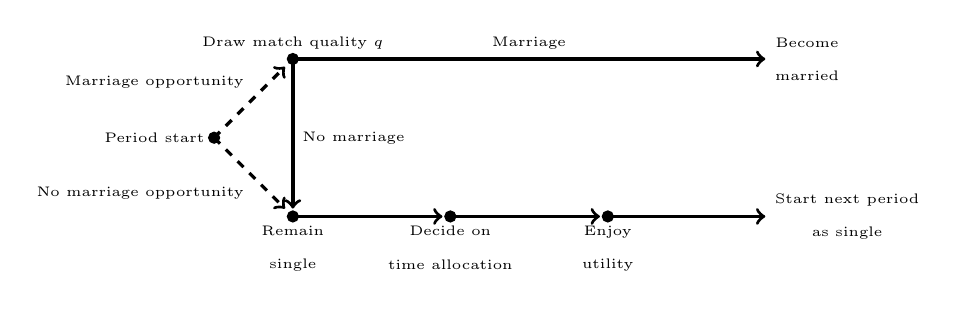
\begin{tikzpicture}
		\node[left] at (0,0) {\tiny Period start};
		\filldraw (0,0) circle (2pt);
		\draw[->, very thick, dashed] (0,0) -- (0.9,0.9);
		\filldraw (1,1) circle (2pt);
		\draw[->, very thick, dashed] (0,0) -- (0.9,-0.9);
		\filldraw (1,-1) circle (2pt);
		\node[align=left, above left] at (0.5,0.5) {\tiny Marriage opportunity};
		\node[align=left, below left] at (0.5,-0.5) {\tiny No marriage opportunity};
		\node[above] at (1,1) {\tiny Draw match quality $q$};
		\draw[->, very thick] (1,1) -- (1,-0.9);
		\node[above] at (4,1) {\tiny Marriage};
		\node[right] at (1,0) {\tiny No marriage};
		\filldraw (3,-1) circle (2pt);
		\node[align=center, below] at (1,-1) {\tiny Remain \\ \tiny single};
		\draw[->, very thick] (1,-1) -- (2.9,-1);
		\node[align=center, below] at (3,-1) {\tiny Decide on \\ \tiny time allocation};
		\draw[->, very thick] (3,-1) -- (4.9,-1);
		\filldraw (5,-1) circle (2pt);
		\node[align=center, below] at (5,-1) {\tiny Enjoy \\ \tiny utility};
		\draw[->, very thick] (5,-1) -- (7,-1);
		\node[align=center, right] at (7,-1) {\tiny Start next period \\ \tiny as single};
		\draw[->, very thick] (1,1) -- (7,1);
		\node[align=center, right] at (7,1) {\tiny Become \\ \tiny married};
		\end{tikzpicture}
	\end{block}
	
	\begin{block}{Married agents}
		\centering
		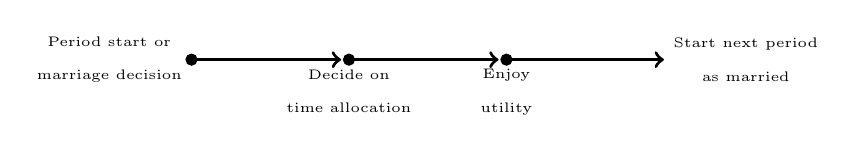
\begin{tikzpicture}
		\node[align=center, left] at (0,0) {\tiny Period start or \\ \tiny marriage decision};
		\filldraw (0,0) circle (2pt);
		\draw[->, very thick] (0,0) -- (1.9,0);
		\node[align=center, below] at (2,0) {\tiny Decide on \\ \tiny time allocation};
		\filldraw (2,0) circle (2pt);
		\draw[->, very thick] (2,0) -- (3.9,0);
		\node[align=center, below] at (4,0) {\tiny Enjoy \\ \tiny utility};
		\filldraw (4,0) circle (2pt);
		\draw[->, very thick] (4,0) -- (6,0);
		\node[align=center, right] at (6,0) {\tiny Start next period \\ \tiny as married};
		\end{tikzpicture}
	\end{block}
	
\end{frame}

\begin{frame}
	\frametitle{Structure of marriage markets for entrants}
	\centering
	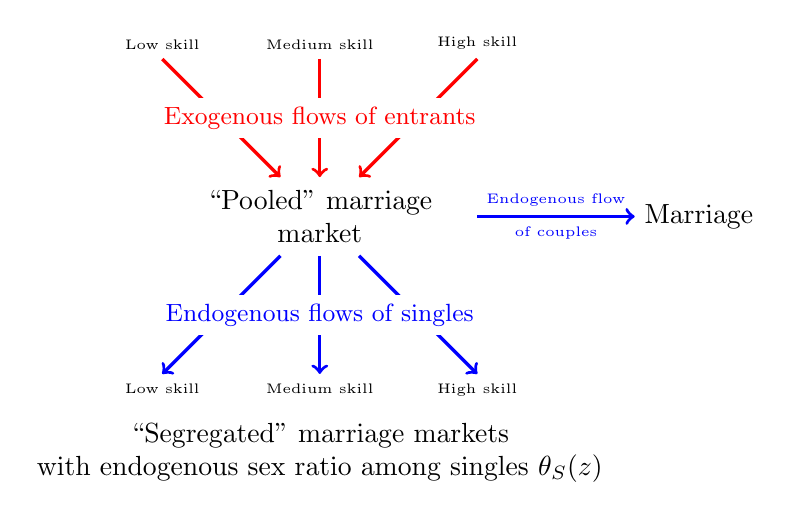
\begin{tikzpicture}
		\node[above] at (-2,2) {\tiny Low skill};
		\draw[->, very thick, red] (-2,2) -- (-0.5,0.5);
		\node[above] at (0,2) {\tiny Medium skill};
		\draw[->, very thick, red] (0,2) -- (0,0.5);
		\node[above] at (2,2) {\tiny High skill};
		\draw[->, very thick, red] (2,2) -- (0.5,0.5);
		\node[align=center, fill=white] at (0,1.25) {\small \textcolor{red}{Exogenous flows of entrants}};
		\node[align=center] at (0,0) {``Pooled'' marriage \\ market};
		\draw[->, very thick, blue] (2,0) -- (4,0);
		\node[right] at (4,0) {Marriage};
		\node[align=center, blue] at (3,0) {\tiny Endogenous flow \\ \tiny of couples};
		\draw[->, very thick, blue] (-0.5,-0.5) -- (-2,-2);
		\node[below] at (-2,-2) {\tiny Low skill};
		\draw[->, very thick, blue] (0,-0.5) -- (0,-2);
		\node[below] at (0,-2) {\tiny Medium skill};
		\draw[->, very thick, blue] (0.5,-0.5) -- (2,-2);
		\node[below] at (2,-2) {\tiny High skill};
		\node[align=center, fill=white] at (0,-1.25) {\small \textcolor{blue}{Endogenous flows of singles}};
		\node[align=center, below] at (0,-2.5) {``Segregated'' marriage markets \\ with endogenous sex ratio among singles $\theta_{S}(z)$};
	\end{tikzpicture}
	
\end{frame}

\begin{frame}
	\frametitle{Meeting probabilities}
	\begin{itemize}
		\item In the ``pooled'' marriage market (only entrants):
		\begin{itemize}
			\item For men: $\frac{1}{\theta_0}$
			\item For women: 1
			\item Conditional on meeting someone, probability of his or her education level to be $z$: $\mathcal{P}_{-i}(z)$
		\end{itemize}
		\item In the ``segregated'' marriage markets:
		\begin{itemize}
			\item For men: $\frac{1}{\theta_{S}(z)}$ if $\theta_{S}(z)>1$, 1 otherwise
			\item For women: $\frac{1}{\theta_{S}(z)}$ if $\theta_{S}(z)<1$, 1 otherwise
		\end{itemize}
	\end{itemize}
\end{frame}

\begin{frame}
	\frametitle{Utility, physical constraints, and technology}
	Utility function:
	\begin{align*}
	u\left(c,l,g\right) = \frac{\sigma_c}{1-\sigma}c^{1-\sigma}+\frac{\sigma_l}{1-\sigma}l^{1-\sigma}+\frac{\sigma_g}{1-\sigma}g^{1-\sigma}
	\end{align*}
	Time constraint:
	\begin{align*}
		l+n+h=1
	\end{align*}
	Home production technology:
	\begin{align*}
	G\left(h,e_q\right) = A_G\left[e_q^{1-\alpha_G}\right]h^{\alpha_G}
	\end{align*}
	Effective housework time for married couples:
	\begin{align*}
	H(h_f,h_m)=\left[\eta_f h_f^{1-\eta}+\left(1-\eta_f\right)h_m^{1-\eta}\right]^{\frac{1}{1-\eta}}.
	\end{align*}
\end{frame}

\begin{frame}
	\frametitle{Single agent's problem}
	
	\begin{align*}
	& \max_{c,l,h,n,e_q,g} u\left(c,l,g\right) \\
	& \text{subject to} \\
	& l+n+h = 1 \\
	& g = G\left(h,e_q\right) \\
	& c = \omega_i\left(z\right)n-p_e e_q
	\end{align*}
	
	Denote the value of the solution of the above problem by $U_i^S\left(z\right)$
	
\end{frame}

\begin{frame}
	\frametitle{Married household's problem}
	\small
	\textcolor{red}{IMPORTANT: the Pareto weight of the wife $\chi_f$ will be an equilibrium object that depends on the conditions of the marriage markets}
		\begin{align*}
		& \max_{c_f,c_m,l_f,l_m,h_m,h_f,n_f,n_m,e_q,g} \left\lbrace \chi_f u_f\left(c_f,l_f,g\right)+\left(1-\chi_f\right) u_m\left(c_m,l_m,g\right) \right\rbrace \\
		& \text{subject to} \\
		& l_f+h_f+n_f = 1 \\
		& l_m+h_m+n_m = 1 \\
		& h = H\left(h_f,h_m\right) \\
		& g = G\left(h,e_q\right) \\
		& c_m+c_f = \omega_f(z_f)n_f+\omega_m(z_m)n_m-p_e e_q
		\end{align*}
		
		Denote the value of the solution of the above problem for an individual of sex $i$  by $U_i^M(z_f,z_m,\chi_f)$
		
\end{frame}

\begin{frame}
	\frametitle{The value of marriage}
	
	Upon meeting, individuals with education levels $z_f$ and $z_m$ draw a match quality $q\sim N\left(\mu_{z_f,z_m},1\right)$. Since $q$ and the wages remain constant in time, in steady state equilibrium there is no divorce, thus:
	
	\begin{align*}
	V_i^M\left(z_f,z_m,\chi_f,q\right)&=\sum_{t=0}^{\infty}\left[\beta\left(1-\delta\right)\right]^t\left[U_i^M(z_f,z_m,\chi_f)+q\right]\\&= \frac{U_i^M(z_f,z_m,\chi_f)+q}{1-\beta\left(1-\delta\right)}
	\end{align*}
\end{frame}

\begin{frame}
	\frametitle{The value of being single}
	\tiny
	The value of remaining single is: 
	\begin{align*}\label{eq:val_single}
	& V_i^S\left(z,\theta_{S}^E(z)\right) = \underbrace{U_i^S\left(z\right)+\psi_i}_{\text{Flow value for singles}} +\underbrace{\beta\left(1-\delta\right)}_{\text{Effective discount rate}}\left\lbrace \rho \underbrace{\frac{U_i^S\left(z\right)+\psi_i}{1-\beta\left(1-\delta\right)}}_{\text{Utility of lifelong single}} \right. \nonumber \\ 
	& \left. + \left(1-\rho\right)\left[ \underbrace{\left[\underbrace{1-\pi_{i}\left(\theta_{S}^E(z)\right)}_{\text{No meeting probability}}+\underbrace{\pi_{i}\left(\theta_{S}^E(z)\right)Q_{z,z}\left[q_r\left(z,z,\theta_{S}^E(z)\right)\right]}_{\text{Meeting but no marriage probability}}\right]}_{\text{Total no marriage probability}}\underbrace{V_i^S\left(z,\theta_{S}^E(z)\right)}_{\text{Value of being single}} \right. \right. \nonumber \\ & \left. \left. + \underbrace{\pi_{i}\left(\theta_{S}^E(z)\right)\underbrace{\left[1-Q_{z,z}\left[q_r\left(z,z,\theta_{S}^E(z)\right)\right]\right]}_{\text{Marriage probability conditional on meeting}}}_{\text{Total marriage probability}}\underbrace{\frac{U_i^M(z,z,\chi_f)+\mathbb{E}\left[q\mid q>q_r\left(z,z,\theta_{S}^E(z)\right)\right]}{1-\beta\left(1-\delta\right)}}_{\text{Expected value of marriage}} \right] \right\rbrace 
	\end{align*}
\end{frame}

\begin{frame}
	\frametitle{Marriage surplus and Egalitarian bargaining}
	
	Marriage between agents with education levels $z_f$ and $z_m$ generates a surplus of:
	\begin{align*}
	W_i\left(z_f,z_m,\chi_f,q,\theta_{S}^E(z)\right) = V_i^M\left(z_f,z_m,\chi_f,q\right)-V_i^S\left(z,\theta_{S}^E(z)\right).
	\end{align*} 
	
	The Pareto weights result from Egalitarian Bargaining, i.e. they are such that:
	
	\begin{align*}
	W_f\left(z_f,z_m,\chi_f,q,\theta_{S}^E(z)\right) = W_m\left(z_f,z_m,\chi_f,q,\theta_{S}^E(z)\right).
	\end{align*}
	
\end{frame}

\begin{frame}
	\frametitle{Equilibrium definition}
	\begin{block}{Steady-state equilibrium with Egalitarian bargaining (SSEB)}
			A SSEB, consists of $q_r\left(z_f,z_m\right)$, $\chi_f(z_f,z_m)$, $V_i^M\left(z_f,z_m,\chi_f,q\right)$, $V_i^S\left(z,\theta_{S}^E(z)\right)$, $\theta_S(z)$ and $\theta_S^E(z)$ for all $\{z_f,z_m\}\in\mathcal{Z}\times\mathcal{Z}$, $z\in\mathcal{Z}$ and $i\in\{f,m\}$ such that: 
			\begin{itemize}
				\item The value functions solve the Bellman equations for men and women.
				\item The reservation match qualities set the marriage surplus to 0.
				\item The allocations implied by the Pareto weights equal those generated by Egalitarian Bargaining.
				\item Expectations are correct: $\theta_{S}^E(z)=\theta_{S}(z)$, $\forall z\in\mathcal{Z}$.
			\end{itemize}
			
	\end{block}

\end{frame}

\section{Calibration}

\begin{frame}
	\frametitle{Calibration strategy}
	
	\begin{itemize}
		\item Objective: choose parameters for the model to replicate the observed time allocation and marital sorting patterns of 1990. 
		\item Three sets of parameters, chosen sequentially:
		\begin{enumerate}
			\item Calibrated externally.
			\item Chosen targeting data moments without having to solve the model.
			\item Chosen targeting data moments in steady-state equilibrium.
		\end{enumerate}
		\item Using said parameters, change the exogenous variables (sex ratio, skill distribution, wages, and home production efficiency and price of home equipment) to 2010 level and assess fit of the model.
	\end{itemize}
\end{frame}

\begin{frame}
	\frametitle{Exogenous objects}
	\tiny
	\begin{table}[]
		\centering
		\caption{Exogenous objects in the model, 1990 and 2010}
		\begin{tabular}{lrrrrrrr}
			\toprule
			\multirow{2}[4]{*}{Classification} & \multicolumn{1}{c}{\multirow{2}[4]{*}{1990}} & \multicolumn{1}{c}{\multirow{2}[4]{*}{2010}} & \multicolumn{2}{c}{Male} &       & \multicolumn{2}{c}{Female} \\
			\cmidrule{4-5}\cmidrule{7-8}      &       &       & 1990  & 2010  &       & 1990  & 2010 \\
			\midrule
			&       &       &       &       &       &       &  \\
			\textit{Sex ratio}, $\theta_0$ & 1.07  & 1.14  & -     & -     &       & -     & - \\
			&       &       &       &       &       &       &  \\
			\textit{Home production} &       &       &       &       &       &       &  \\
			$p_e$ & 1.82  & 1.06  & -     & -     &       & -     & - \\
			\textit{$A_g$} & 1.00  & 6.23  & -     & -     &       & -     & - \\
			&       &       &       &       &       &       &  \\
			\textit{Skill distribution} &       &       &       &       &       &       &  \\
			Low skill & -     & -     & 0.33  & 0.14  &       & 0.47  & 0.18 \\
			Medium Skill & -     & -     & 0.63  & 0.58  &       & 0.49  & 0.51 \\
			High skill & -     & -     & 0.04  & 0.29  &       & 0.04  & 0.31 \\
			&       &       &       &       &       &       &  \\
			\textit{Wages} &       &       &       &       &       &       &  \\
			Low skill & -     & -     & 1.00  & 2.35  &       & 0.83  & 1.77 \\
			Medium Skill & -     & -     & 1.06  & 2.88  &       & 0.89  & 2.16 \\
			High skill & -     & -     & 1.29  & 4.37  &       & 1.07  & 3.29 \\
			\bottomrule
			\bottomrule
		\end{tabular}
	\end{table}
\end{frame}

\begin{frame}
	\frametitle{Calibrated model parameters}
	\tiny
	\begin{table}[htbp]
		\centering
		\caption{Calibrated parameters I}
		\begin{tabular}{lll}
			\toprule
			\multicolumn{3}{c}{Parameters externally calibrated} \\
			\midrule
			Parameter & Value & Source \\
			\midrule
			$\beta$ & \multicolumn{1}{r}{0.960} & Standard \\
			$\delta$ & \multicolumn{1}{r}{0.020} & Life expectancy of 49 years \\
			$\rho$ & \multicolumn{1}{r}{0.067} & Expected 15 years searching for spouse \\
			$\sigma$ & \multicolumn{1}{r}{1.250} & Midpoint between Attanasio et. al (2008) and 1 \\
			$\alpha_g$ & \multicolumn{1}{r}{0.950} & Knowles (2014) \\
			$\eta$ & \multicolumn{1}{r}{0.330} & Knowles (2014) \\
			\midrule
			\multicolumn{3}{c}{Parameters calibrated before solving the model} \\
			\midrule
			Parameter & Value & Set to match \\
			\midrule
			$\eta_f$ & \multicolumn{1}{r}{0.580} & Gender housework ratio, married people in 1990 \\
			\multicolumn{2}{l}{\textit{Single women}} &  \\
			$\sigma_c$ & \multicolumn{1}{r}{0.391} &  \\
			$\sigma_l$ & \multicolumn{1}{r}{0.570} & Single women time allocation \\
			$\sigma_g$ & \multicolumn{1}{r}{0.040} &  \\
			\multicolumn{2}{l}{\textit{Single men}} &  \\
			$\sigma_c$ & \multicolumn{1}{r}{0.387} &  \\
			$\sigma_l$ & \multicolumn{1}{r}{0.607} & Single men time allocation \\
			$\sigma_g$ & \multicolumn{1}{r}{0.006} &  \\
			\bottomrule
			\bottomrule
		\end{tabular}
	\end{table}
\end{frame}

\begin{frame}
	\frametitle{Calibrated model parameters}
	\tiny
		\begin{table}[htbp]
		\centering
		\caption{Calibrated parameters II}
		\begin{tabular}{lll}
			\toprule
			\multicolumn{3}{c}{Parameters jointly calibrated by moment matching in steady-state} \\
			\midrule
			Parameter & Value & Target \\
			\midrule
			\multicolumn{2}{l}{\textit{Married people}} &  \\
			$\sigma_c$ & \multicolumn{1}{r}{0.365} &  \\
			$\sigma_l$ & \multicolumn{1}{r}{0.573} & \multicolumn{1}{p{20.68em}}{Married households time allocation} \\
			$\sigma_g$ & \multicolumn{1}{r}{0.062} &  \\
			$\psi_f$ & \multicolumn{1}{r}{-0.373} & Husband to wife leisure ratio \\
			$M$ & See Table below & Marital sorting contingency matrix \\
			\bottomrule
			\bottomrule
		\end{tabular}
	\end{table}
	\begin{table}[]
	\centering
	\caption{Means of the match quality draws ($M$)}
	\begin{tabular}{lrrr}
		\toprule
		\multicolumn{1}{c}{\multirow{2}[4]{*}{Female skill level}} & \multicolumn{3}{c}{Male skill level} \\
		\cmidrule{2-4}          & \multicolumn{1}{l}{Low} & \multicolumn{1}{l}{Medium} & \multicolumn{1}{l}{High} \\
		\midrule
		Low   & 0.753 & 1.483 & -0.004 \\
		Medium & 0.813 & -0.253 & 4.078 \\
		High  & -0.698 & 0.608 & -0.785 \\
		\bottomrule
		\bottomrule
	\end{tabular}
	\end{table}
\end{frame}

\begin{frame}
	\frametitle{Calibration results, time allocation}
	\scriptsize
	\begin{table}[htbp]
		\centering
		\caption{Time allocation 1990, model and data (hours per week)}
		\begin{tabular}{lrr}
			\toprule
			Statistic & \multicolumn{1}{l}{Model} & \multicolumn{1}{l}{Data} \\
			\midrule
			Married women housework & 18.09 & 18.13 \\
			Married women paid work & 41.10 & 41.06 \\
			Married women leisure & 58.82 & 58.81 \\
			Married men housework & 3.91  & 3.81 \\
			Married men paid work & 47.38 & 47.48 \\
			Married men leisure & 66.71 & 66.71 \\
			Single women housework & 7.39  & 7.39 \\
			Single women paid work & 48.00 & 48.01 \\
			Single women leisure & 62.61 & 62.60 \\
			Single men housework & 1.66  & 1.66 \\
			Single men paid work & 47.55 & 47.56 \\
			Single men leisure & 68.79 & 68.78 \\
			\bottomrule
			\bottomrule
		\end{tabular}
	\end{table}
\end{frame}

\begin{frame}
	\frametitle{Calibration results, marital sorting}\label{frame:calib_results_ms}
	\scriptsize
	\begin{table}[]
		\centering
		\caption{Marital sorting 1990, model and data}
		\begin{tabular}{lcccccccc}
			\toprule
			\multicolumn{1}{c}{\multirow{3}[6]{*}{Wife}} & \multicolumn{8}{c}{Husband} \\
			\cmidrule{2-9}          & \multicolumn{2}{c}{Low skill} &       & \multicolumn{2}{c}{Medium skill} &       & \multicolumn{2}{c}{High skill} \\
			\cmidrule{2-3}\cmidrule{5-6}\cmidrule{8-9}          & Data  & Model &       & Data  & Model &       & Data  & Model \\
			\midrule
			Low skill & 0.251 & 0.263 &       & 0.247 & 0.206 &       & 0.006 & 0.004 \\
			Medium skill & 0.074 & 0.072 &       & 0.371 & 0.400 &       & 0.023 & 0.022 \\
			High skill & 0.001 & 0.001 &       & 0.011 & 0.013 &       & 0.017 & 0.020 \\
			\bottomrule
			\bottomrule
		\end{tabular}
	\end{table}
	
	\begin{itemize}
		\item Assortative mating data: 1.39
		\item Assortative mating model: 1.46
	\end{itemize}

	\hyperlink{appendix:ct_approach}{\beamergotobutton{Contingency table approach}}	
\end{frame}

\begin{frame}
	\frametitle{Model fit, time allocation}
	\scriptsize
	\begin{table}[htbp]
		\centering
		\caption{Time allocation 2010, model and data}
			\begin{tabular}{lrrrrr}
				\toprule
				\multirow{2}[4]{*}{Statistic} & \multicolumn{2}{c}{Hours per week} &       & \multicolumn{2}{c}{$\Delta$\% 1990-2010} \\
				\cmidrule{2-3}\cmidrule{5-6}      & \multicolumn{1}{l}{Data} & \multicolumn{1}{l}{Model} &       & \multicolumn{1}{l}{Data} & \multicolumn{1}{l}{Model} \\
				\midrule
				Married women housework & 11.27 & 15.06 &       & -47.32\% & -18.58\% \\
				Married women paid work & 35.87 & 31.59 &       & -13.61\% & -26.22\% \\
				\textcolor[rgb]{ 1,  0,  0}{\textbf{Married women leisure}} & \textcolor[rgb]{ 1,  0,  0}{\textbf{70.86}} & \textcolor[rgb]{ 1,  0,  0}{\textbf{71.36}} & \textcolor[rgb]{ 1,  0,  0}{} & \textcolor[rgb]{ 1,  0,  0}{\textbf{18.64\%}} & \textcolor[rgb]{ 1,  0,  0}{\textbf{19.34\%}} \\
				Married men housework & 2.70  & 2.56  &       & -37.02\% & -39.67\% \\
				Married men paid work & 47.51 & 45.42 &       & 0.28\% & -4.44\% \\
				Married men leisure & 67.79 & 70.02 &       & 1.60\% & 4.84\% \\
				Single women housework & 4.50  & 5.54  &       & -49.69\% & -28.75\% \\
				Single women paid work & 45.06 & 43.31 &       & -6.32\% & -10.31\% \\
				Single women leisure & 68.44 & 69.15 &       & 8.91\% & 9.95\% \\
				Single men housework & 1.59  & 1.23  &       & -4.68\% & -30.02\% \\
				Single men paid work & 42.73 & 41.68 &       & -10.70\% & -13.19\% \\
				Single men leisure & 73.69 & 75.09 &       & 6.88\% & 8.78\% \\
				\bottomrule
				\bottomrule
			\end{tabular}
	\end{table}
\end{frame}

\begin{frame}
	\frametitle{Model fit, marital sorting}\label{frame:fit_ms}
	\scriptsize
	\begin{table}[]
		\centering
		\caption{Marital sorting 2010, model and data}
		\begin{tabular}{lcccccccc}
			\toprule
			\multicolumn{1}{c}{\multirow{3}[6]{*}{Wife}} & \multicolumn{8}{c}{Husband} \\
			\cmidrule{2-9}          & \multicolumn{2}{c}{Low skill} &       & \multicolumn{2}{c}{Medium skill} &       & \multicolumn{2}{c}{High skill} \\
			\cmidrule{2-3}\cmidrule{5-6}\cmidrule{8-9}          & Data  & Model &       & Data  & Model &       & Data  & Model \\
			\midrule
			Low skill & 0.099 & 0.100 &       & 0.101 & 0.072 &       & 0.002 & 0.010 \\
			Medium skill & 0.051 & 0.036 &       & 0.433 & 0.362 &       & 0.068 & 0.143 \\
			High skill & 0.005 & 0.005 &       & 0.079 & 0.114 &       & 0.162 & 0.158 \\
			\bottomrule
			\bottomrule
		\end{tabular}
	\end{table}

	\begin{itemize}
	\item Assortative mating data: 1.62
	\item Assortative mating model: 1.52
	\end{itemize}

	\hyperlink{appendix:ct_approach}{\beamergotobutton{Contingency table approach}}
\end{frame}

\section{Quantitative experiments}

\begin{frame}
	\frametitle{Decomposition: married women's time allocation}\label{slide:decomp_female_ta}
	\begin{figure}[hp]
		\centering
		\caption{Contributions to changes in married women's time allocation, 1990-2010}
		\includegraphics[width=.6\textwidth]{for_decomp_ta_f}
	\end{figure}
	\hyperlink{slide:decomp_female_ta_back}{\beamergotobutton{Backward decomposition}}
\end{frame}

\begin{frame}
	\frametitle{Decomposition: married men's time allocation}
	\begin{figure}[hp]
		\centering
		\caption{Contributions to changes in married men's time allocation, 1990-2010}\label{slide:decomp_male_ta}
		\includegraphics[width=.6\textwidth]{for_decomp_ta_m}
	\end{figure}
	\hyperlink{slide:decomp_male_ta_back}{\beamergotobutton{Backward decomposition}}
\end{frame}

\begin{frame}
	\frametitle{Decomposition: assortative mating}\label{slide:decomp_ms}
	\begin{figure}[hp]
		\centering
		\caption{Contributions to changes in assortative mating, 1990-2010}
		\includegraphics[width=.6\textwidth]{for_decomp_ms}
	\end{figure}
	\hyperlink{slide:decomp_ms_back}{\beamergotobutton{Backward decomposition}}
\end{frame}

\begin{frame}
	\frametitle{Further decomposition: bargaining versus marital sorting channel}
	\begin{table}[htbp]
		\centering
		\caption{Decomposition of the effect of the sex ratio on time allocation for married people}
		\begin{tabular}{lrr}
			\toprule
			Statistic & \multicolumn{1}{l}{Bargaining} & \multicolumn{1}{l}{Sorting} \\
			\midrule
			Married women housework & -44.10\% & -55.90\% \\
			Married women paid work & -105.15\% & 5.15\% \\
			Married women leisure & 104.27\% & -4.27\% \\
			Married men housework & -96.98\% & 196.98\% \\
			Married men paid work & 104.35\% & -4.35\% \\
			Married men leisure & -104.54\% & 4.54\% \\
			\bottomrule
			\bottomrule
		\end{tabular}
	\end{table}
\end{frame}

\begin{frame}
	\frametitle{A sex ratio of 1.2}
	\scriptsize
	\begin{table}[htbp]
		\centering
		\caption{The effects of a sex ratio of 1.2 in 2010}
		\begin{tabular}{lrrr}
			\toprule
			Statistic & \multicolumn{1}{l}{Baseline 2010} & \multicolumn{1}{l}{$\theta_0=1.2$} & \multicolumn{1}{l}{\% change} \\
			\midrule
			&       &       &  \\
			Married women housework & 15.06 & 14.97 & -0.54\% \\
			\textcolor[rgb]{ 1,  0,  0}{\textbf{Married women paid work}} & \textcolor[rgb]{ 1,  0,  0}{\textbf{31.59}} & \textcolor[rgb]{ 1,  0,  0}{\textbf{28.90}} & \textcolor[rgb]{ 1,  0,  0}{\textbf{-8.90\%}} \\
			Married women leisure & 71.36 & 74.13 & 3.81\% \\
			Married men housework & 2.56  & 2.58  & 0.91\% \\
			Married men paid work & 45.42 & 47.81 & 5.12\% \\
			Married men leisure & 70.02 & 67.61 & -3.50\% \\
			&       &       &  \\
			Married women consumption & 0.83  & 0.87  & 4.65\% \\
			Married men consumption & 1.08  & 1.05  & -3.14\% \\
			&       &       &  \\
			Average wife Pareto weight & 0.44  & 0.46  & 5.35\% \\
			&       &       &  \\
			Assortative mating measure & 1.52  & 1.55  & 2.15\% \\
			\bottomrule
			\bottomrule
		\end{tabular}
	\end{table}
\end{frame}

\begin{frame}
	\frametitle{The role of the gender wage gap}
	\scriptsize
	\begin{table}[htbp]
		\centering
		\caption{The model in 2010 with no gender wage gap}
		\begin{tabular}{lrrr}
			\toprule
			Statistic & \multicolumn{1}{l}{Baseline 2010} & \multicolumn{1}{l}{No gender wage gap} & \multicolumn{1}{l}{\% change} \\
			\midrule
			&       &       &  \\
			Married women housework & 15.06 & 11.82 & -24.17\% \\
			\textcolor[rgb]{ 1,  0,  0}{\textbf{Married women paid work}} & \textcolor[rgb]{ 1,  0,  0}{\textbf{31.59}} & \textcolor[rgb]{ 1,  0,  0}{\textbf{34.37}} & \textcolor[rgb]{ 1,  0,  0}{\textbf{8.45\%}} \\
			Married women leisure & 71.36 & 71.80 & 0.63\% \\
			Married men housework & 2.56  & 4.50  & 56.41\% \\
			Married men paid work & 45.42 & 42.81 & -5.91\% \\
			Married men leisure & 70.02 & 70.68 & 0.95\% \\
			&       &       &  \\
			Married women consumption & 0.83  & 1.04  & 22.51\% \\
			Married men consumption & 1.08  & 1.09  & 1.12\% \\
			&       &       &  \\
			Average wife Pareto weight & 0.44  & 0.50  & 14.10\% \\
			&       &       &  \\
			Assortative mating measure & 1.52  & 1.52  & 0.16\% \\
			\bottomrule
			\bottomrule
		\end{tabular}
	\end{table}
\end{frame}

\section{Conclusions}

\begin{frame}
	\frametitle{Conclusions}
	\begin{itemize}
		\item Built a model of marriage and time allocation that features endogenous marital sorting and bargaining between spouses
		\item Calibrated said model to Chinese data 
		\item Found that the sex ratio explains a significant fraction of the changes in time allocation for married people, especially on paid work and leisure
		\item Moreover that the effect of the sex ratio works mainly through bargaining instead of marital sorting
		\item Eliminating the gender wage gap offsets the reduction of the increasing sex ratio on female labor supply
		\item Further work: explore other bargaining solutions (Nash), make education decisions endogenous
	\end{itemize}
\end{frame}

\appendix

\begin{frame}[noframenumbering]
	\frametitle{Leisure ratio}\label{appendix:leisure_ratio}
	\begin{figure}
		\centering
		\caption{Leisure ratio by marital stauts among Chinese people aged 20-35, 1990-2010}
		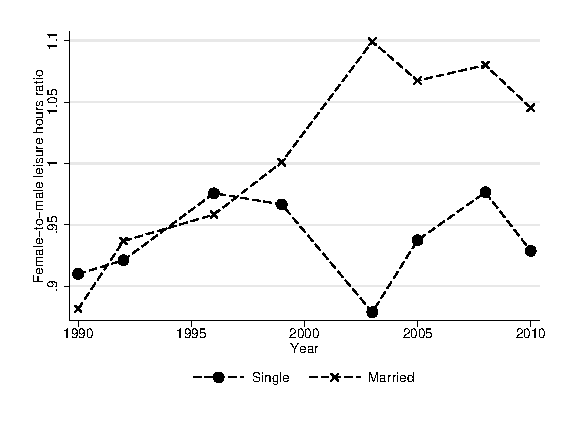
\includegraphics[width=.6\textwidth]{leisure_ratio_all}
	\end{figure}
	\hyperlink{frame:time_allocation}{\beamerreturnbutton{Changes in time allocation patterns}}
\end{frame}

\begin{frame}[noframenumbering]
	\frametitle{China's increasingly unbalanced sex ratio}\label{slide:sex_ratio_20_35}
	\begin{figure}[]
		\centering
		\caption{Sex ratio in China for population aged 20-35, 1990-2020}
		\includegraphics[width=.6\textwidth]{sex_ratio_20_35}
		\source{Projected from the 2000 Population Census.}
	\end{figure}
	\hyperlink{slide:sex_ratio_birth}{\beamerreturnbutton{Sex ratio at birth}}
\end{frame}

\begin{frame}
	\scriptsize
	\frametitle{Wage structure}\label{appendix:wage_struct}
	\begin{table}[htbp]
		\centering
		\caption{Changes in wage structure in China, 1992-2007}
		\begin{tabular}{lrrr}
			\toprule
			& \multicolumn{1}{c}{Annual growth} & \multicolumn{2}{c}{Premium} \\
			\cmidrule{3-4}Classification & \multicolumn{1}{c}{1992-2007} & 1992  & 2007 \\
			\midrule
			Overall & 7.6\% &   -    & - \\
			&       &       &  \\
			By skill &       &       &  \\
			Low   & 5.9\% &   -    & - \\
			Medium & 6.9\% & 6.44\% & 22.46\% \\
			High  & 8.5\% & 28.63\% & 86.08\% \\
			&       &       &  \\
			By sex &       &       &  \\
			Female & 7.2\% &   -    & - \\
			Male  & 7.9\% & 20.01\% & 33.04\% \\
			\bottomrule
			\bottomrule
		\end{tabular}
		\source{Author's calculations using the data presented in Table 1 of Ge \& Tao (2014).}
	\end{table}
	\hyperlink{appendix:skill_premium_chns}{\beamergotobutton{Skill premium in the CHNS}}
	\hyperlink{appendix:gender_wage_ratio_chns}{\beamergotobutton{Gender wage ratio in the CHNS}}
\end{frame}

\begin{frame}[noframenumbering]
	\frametitle{Skill premium in the CHNS}\label{appendix:skill_premium_chns}
	\begin{figure}[hp]
		\centering
		\caption{Skill premium in China by sex, 1990 and 2010}
		\subfloat[Women]{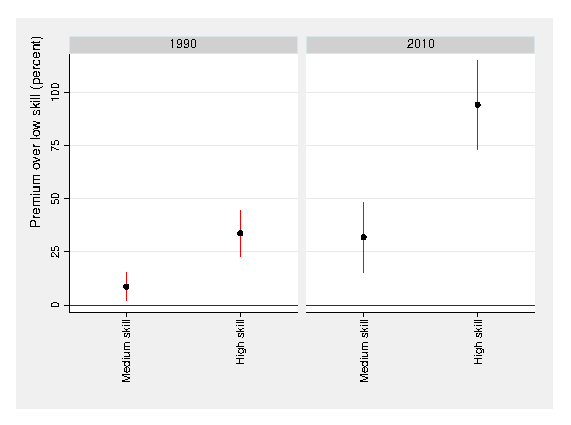
\includegraphics[width=.4\textwidth]{skill_premium_women}}
		~
		\subfloat[Men]{\includegraphics[width=.4\textwidth]{skill_premium_men}}
		\source{Author's calculations using the China Health and Nutrition Survey.}
	\end{figure}
	\hyperlink{appendix:wage_struct}{\beamerreturnbutton{Wage structure}}
\end{frame}

\begin{frame}[noframenumbering]
	\frametitle{The gender wage ratio in the CHNS}\label{appendix:gender_wage_ratio_chns}
	\begin{figure}
		\centering
		\caption{Gender wage ratio in China, 1990-2010}
		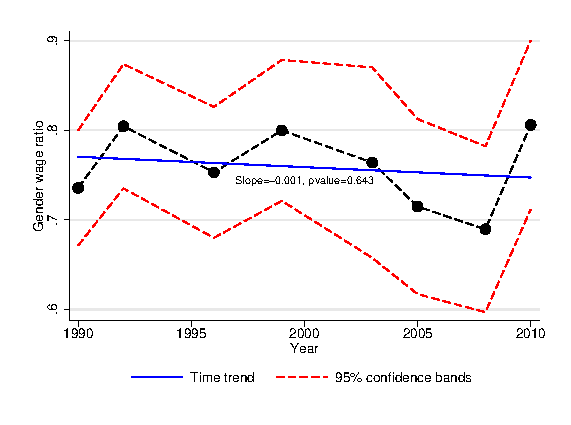
\includegraphics[width=.6\textwidth]{gender_wage_ratio}
		\source{Author's calculations using the China Health and Nutrition Survey.}
	\end{figure}
	\hyperlink{appendix:wage_struct}{\beamerreturnbutton{Wage structure}}
\end{frame}

\begin{frame}
	\frametitle{Assortative mating}\label{appendix:assortative_mating}
	\begin{figure}[]
		\centering
		\caption{Assortative mating in China among people aged 20-35, 1990-2010}\label{fig:assortative_mating}
		\subfloat[Regression approach]{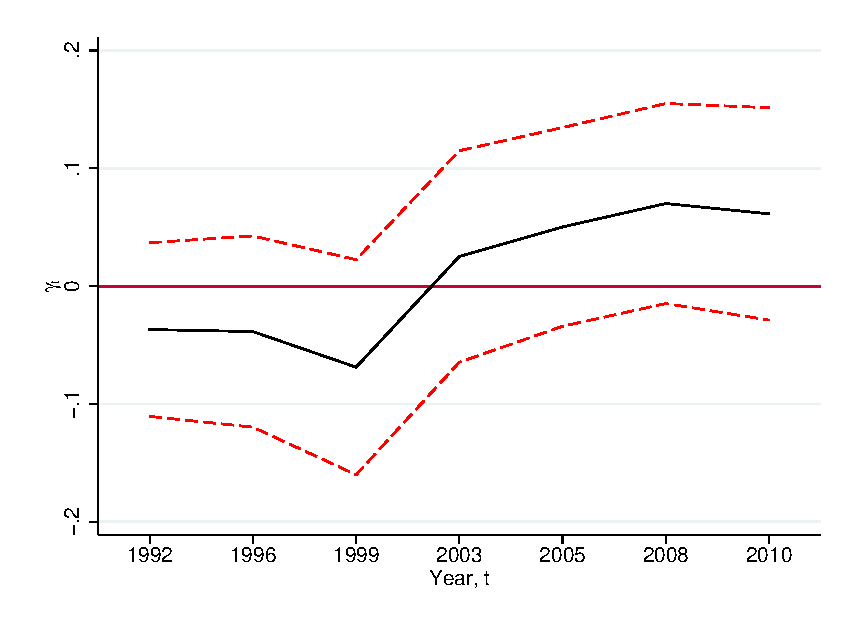
\includegraphics[width=.3\textwidth]{gammas}}
		~
		\subfloat[Rank correlation approach]{\includegraphics[width=.3\textwidth]{kendallstau}}
		~
		\subfloat[Contingency table approach]{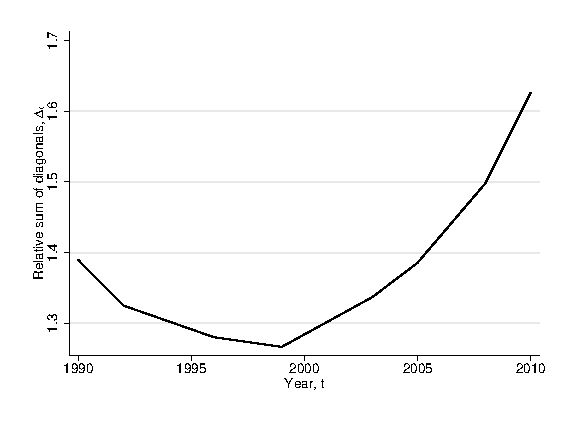
\includegraphics[width=.3\textwidth]{deltas}}
	\end{figure}
	\hyperlink{appendix:reg_approach}{\beamergotobutton{Regression approach}}
	\hyperlink{appendix:ct_approach}{\beamergotobutton{Contingency table approach}}
\end{frame}

\begin{frame}[noframenumbering]
	\frametitle{Assortative mating measures: regression approach}\label{appendix:reg_approach}
	\footnotesize
	I regress wife's education level on her husband's:
	\begin{align*}
	EDU_{my}^w = \alpha + \beta\times EDU_{my}^h+\sum_{t\in T} \gamma_t\times EDU_{my}^h\times YEAR_{ty}+\sum_{t\in T}\theta_t\times YEAR_{ty}+\epsilon_{my}
	\end{align*}
	
	I am interested in the $\gamma_t$'s which measure the difference between wife and husband's correlation in year $t$ and the baseline year. If $\gamma_t$ rises with $t$, there's evidence of increasing assortative mating over time.
	
	\hyperlink{appendix:assortative_mating}{\beamerreturnbutton{Assortative mating}}	
\end{frame}

\begin{frame}[noframenumbering]
	\frametitle{Assortative mating measures: contingency table approach}\label{appendix:ct_approach}
	\tiny
	\begin{table}[htbp]
		\centering
		\caption{Contingency matrix, 1990}
		\begin{tabular}{lccrccrccrr}
			\toprule
			\multicolumn{1}{c}{\multirow{2}[4]{*}{Wife}} & \multicolumn{10}{c}{Husband} \\
			\cmidrule{2-11}          & \multicolumn{2}{c}{Low skill} &       & \multicolumn{2}{c}{Medium skill} &       & \multicolumn{2}{c}{High skill} &       & \multicolumn{1}{l}{Marginal} \\
			\midrule
			Low skill & \textcolor[rgb]{ .753,  0,  0}{\textbf{0.251}} & \textcolor[rgb]{ 0,  .439,  .753}{\textbf{0.164}} &       & 0.247 & 0.317 &       & 0.006 & 0.023 &       & 0.504 \\
			Medium skill & 0.074 & 0.153 &       & \textcolor[rgb]{ .753,  0,  0}{\textbf{0.371}} & \textcolor[rgb]{ 0,  .439,  .753}{\textbf{0.294}} &       & 0.023 & 0.021 &       & 0.468 \\
			High skill & 0.001 & 0.009 &       & 0.011 & 0.018 &       & \textcolor[rgb]{ .753,  0,  0}{\textbf{0.017}} & \textcolor[rgb]{ 0,  .439,  .753}{\textbf{0.001}} &       & 0.028 \\
			Marginal & \multicolumn{2}{c}{0.326} &       & \multicolumn{2}{c}{0.629} &       & \multicolumn{2}{c}{0.046} &       &  \\
			\bottomrule
			\bottomrule
		\end{tabular}
	\end{table}
	
	\begin{align*}
		\Delta_{1990}=\frac{\text{\textcolor{red}{0.251+0.371+0.017}}}{\text{\textcolor{blue}{0.164+0.294+0.001
		}}}=1.39
	\end{align*}
		
	\hyperlink{appendix:assortative_mating}{\beamerreturnbutton{Assortative mating}}
	\hyperlink{frame:calib_results_ms}{\beamerreturnbutton{Calibration results: marital sorting}}
	\hyperlink{frame:fit_ms}{\beamerreturnbutton{Fit: marital sorting}}
\end{frame}

\begin{frame}[noframenumbering]
	\frametitle{Decomposition: married women's time allocation (backward)}\label{slide:decomp_female_ta_back}
	\begin{figure}
		\centering
		\caption{Contributions to changes in married women's time allocation, 1990-2010}
		\includegraphics[width=.6\textwidth]{back_decomp_ta_f}
	\end{figure}
	\hyperlink{slide:decomp_female_ta}{\beamergotobutton{Forward decomposition}}
\end{frame}

\begin{frame}[noframenumbering]
	\frametitle{Decomposition: married men's time allocation (backward)}\label{slide:decomp_male_ta_back}
	\begin{figure}
		\centering
		\caption{Contributions to changes in married men's time allocation, 1990-2010}
		\includegraphics[width=.6\textwidth]{back_decomp_ta_f}
	\end{figure}
	\hyperlink{slide:decomp_male_ta}{\beamergotobutton{Forward decomposition}}
\end{frame}

\begin{frame}[noframenumbering]
	\frametitle{Decomposition: assortative mating (backward)}\label{slide:decomp_ms_back}
	\begin{figure}
		\centering
		\caption{Contributions to changes in assortative mating, 1990-2010}
		\includegraphics[width=.6\textwidth]{back_decomp_ms}
	\end{figure}
	\hyperlink{slide:decomp_ms}{\beamergotobutton{Forward decomposition}}
\end{frame}

\end{document}